\documentclass[12pt]{article}

% Load necessary packages
\usepackage{geometry}
\usepackage{setspace}
\usepackage{natbib}
\usepackage{graphicx}
\usepackage{amsmath}
\usepackage{amssymb}
\usepackage{caption}
\usepackage{subcaption}
\usepackage{hyperref}

% Set page margins
\geometry{margin=1in}

% Set line spacing
\doublespacing

% Title and author information
\title{Exploring the relationship between mother household headship and child vaccination rate in Nepal
}
\author{Prabidhik KC\thanks{Harvard University, Cambridge, USA. Email: \href{mailto:prabidhik_kc@college.harvard.edu}{prabidhik_kc@college.harvard.edu}}}

% Date
\date{May 7, 2023}

\begin{document}

% Title page
\maketitle

% Abstract
\begin{abstract}
I exploit the differences in family member absentees caused by the foreign employement to estimate the effect of mother household headship on child vaccination rate. Using instrumental variable method and data from Nepal Social Inclusion Survey (NSIS) 2018, I find that there is no statistically significant affect on child vaccination rate if the household head is mother instead of father. Even after controlling for education, log wage, ethnicity, I do not find any significant effect in bacterial vaccination and viral vaccination.
\end{abstract}

% Introduction
\section{Introduction}
In low income countries, communicable disease is far more likely to be a cause of death than a noncommunicable disease. 6 of the top 10 causes of death remain such communicable diseases in low income countries, with Tuberculosis, HIV/AIDS and malaria all remaining in the top 10 (WHO, 2019). Thus, childhood vaccination is a crucial component of public health programs especially as a profound measure to reduce deaths from such diseases, notably in the developing countries like Nepal. According to Ministry of Health and Population, Nepal started providing BCG vaccine to all infants in free of cost (National Immunization Program) since 2005, pneumococcal vaccine since  2019, Oral Polio and DPT since 1979, Rubella in 2018. Despite this availability of free vaccines, the vaccinations coverage in Nepal is not yet full capacity, shown in the map of Nepal below in two categories: viral vaccination which includes Oral Polio, DPT, and Rubella and bacterial vaccine which includes BCG and Pneumococcal vaccine, with each 14 zones: the zone Karnali is not included because of lack of data, which puts children at a risk of preventable diseases. Previous researches have identified various factors that affects vaccination rates including socioeconomic conditions, maternal education, access to health care to mention few. However, the impact of maternal headship on vaccination rate has received less attention in the literature. This research aims to fill this gap by examining whether mother as a household head affects child vaccination rate in Nepal, using Nepal Inclusion Social Survey (NSIS) 2018. The findings of this study will provide insights into the role of household headship improving vaccination coverage and inform policies to promote child health care in Nepal.


\begin{figure}[h]
    \centering
    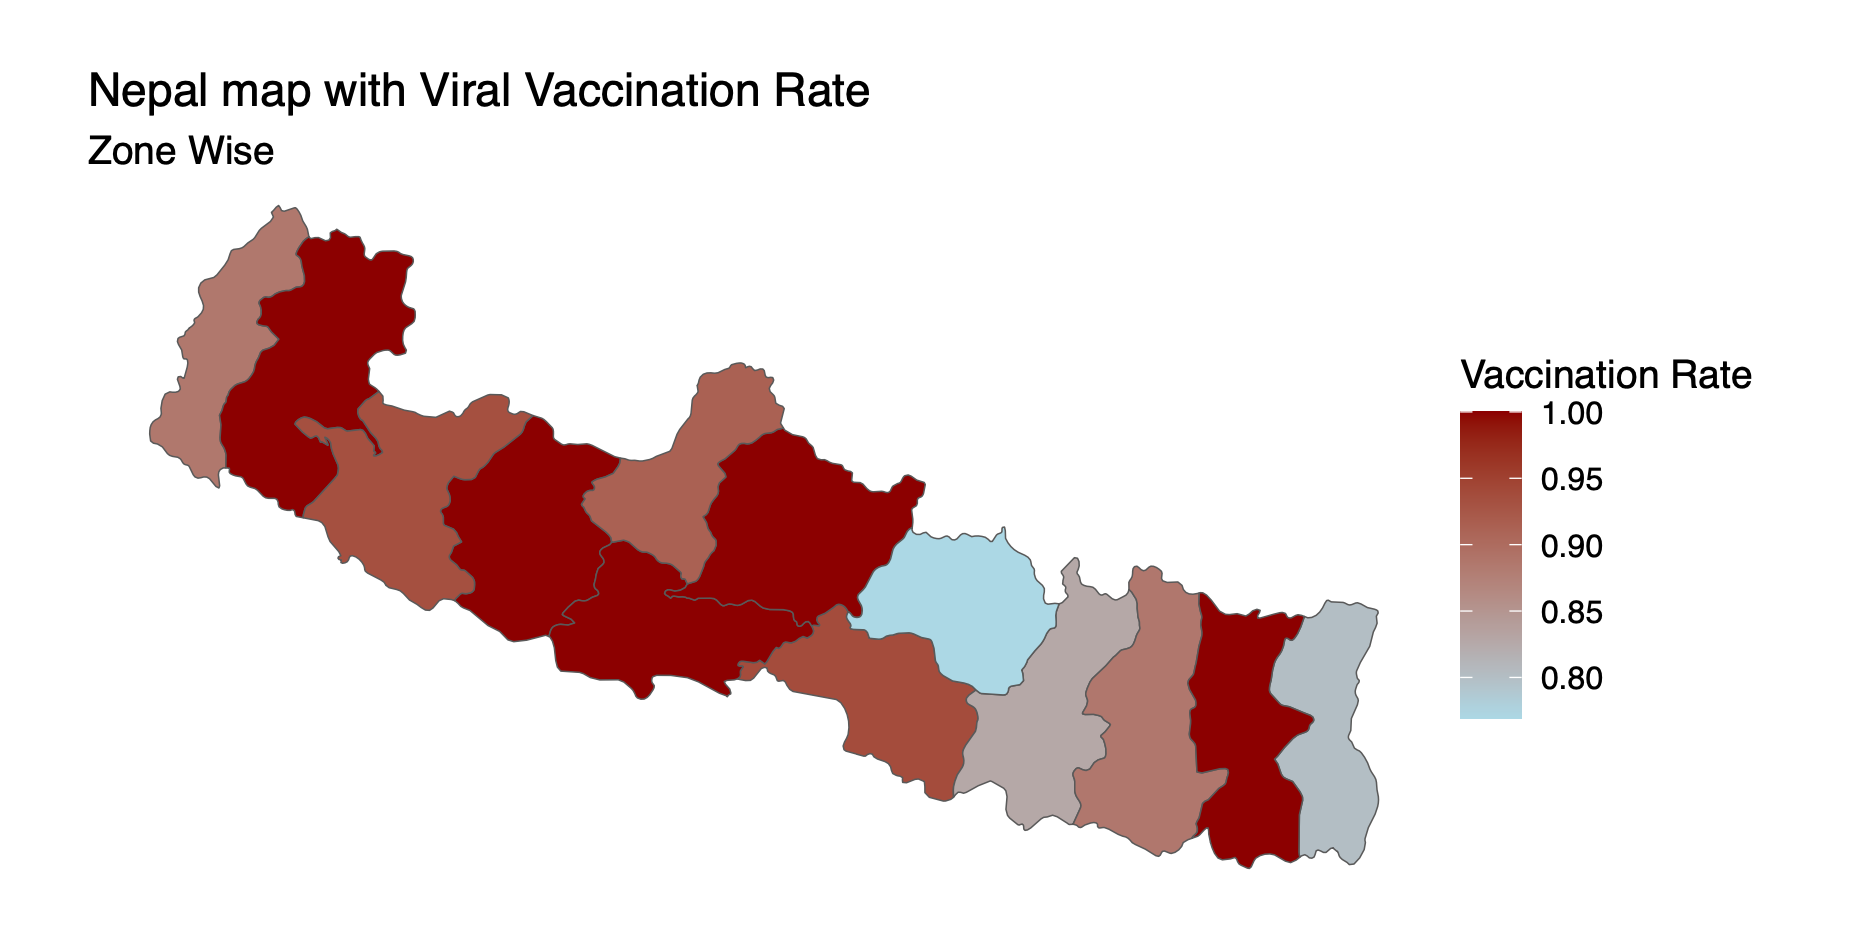
\includegraphics[width=1\textwidth]{viral.png}
    \caption{Viral Vaccination rate in different zones of Nepal}
    \label{Viral Vaccination rate in different zones of Nepal}
\end{figure}

\begin{figure}[h]
    \centering
    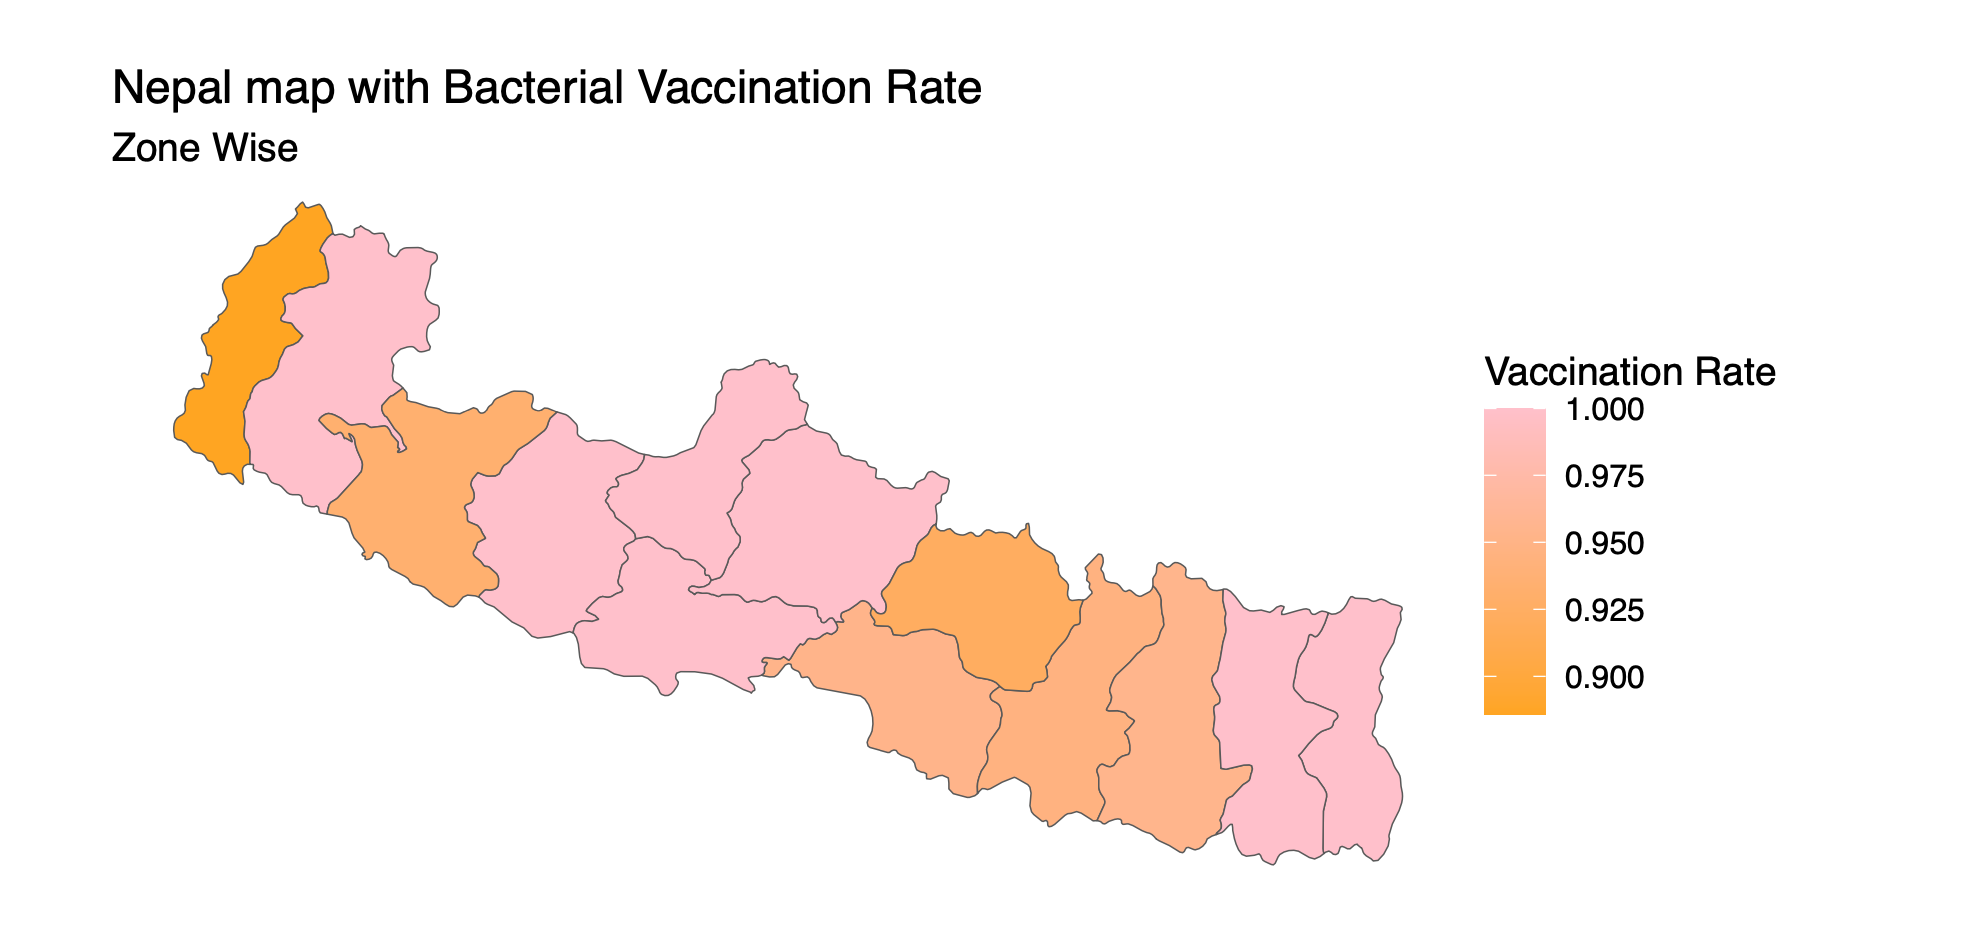
\includegraphics[width=1\textwidth]{bacterial.png}
    \caption{Bacterial Vaccination rate in different zones of Nepal}
    \label{Bacterial Vaccination rate in different zones of Nepal}
\end{figure}

% Literature Review
\section{Literature Review}
Vaccination is a pivotal preventive measure, particularly for the children, as it helps them protect them against several diseases. The World Health Organization estimates that the vaccination prevents approximately 2-3 million deaths per year. However, despite these proven efficacy of vaccines, there are still gaps in vaccination coverages in many parts of the world, specifically in low and middle income countries (Yousufzhai et. al, 2018). Nepal is one such country where vaccination rates are still low with only 77\% of children, as shown in the map above, aged 12-23 months having received all the vaccinations (Ministry of Health and Population, 2019).

The literature on the relationship between household headship and child health outcomes is mixed. Some studies suggest that having a female household headship is associated with a lower child vaccination rate due to socioeconomic status and limited access to health care services (Burgard \& reiman, 2006; Fulu et al., 2017, Sharma \& Reichenbach, 2018). 

In the context of Nepal, few studies have examined the relationship between the household headship and child vaccination rates. One study found that household with female headship were less likely to vaccinate their children due to lower education level and socioeconomic status (Kamiya et. al, 2017). However, this study did not control for other important factors that may have influenced vaccination rate such as access to health care and maternal-decision making power. Therefore, further research is necessary to understand the household headship and children vaccination rate in Nepal.

The NSIS data from 2018 provides us a unique opportunity to examine this relationship. The dataset includes detail information on household composition, socioeconomic status, and child health outcomes, absentee population allowing for the comprehensive analysis of the factors related with the child vaccination rate. By exploring the relationship between household headship and child vaccinations rate in Nepal, this research aims to provide valuable insights into the factors that affect child vaccination rate.


% Data 
\section{Data}
In my study, I use data from Nepal Social Inclusion Survey (NSIS) 2018. NSIS is a survey dataset which is conducted as a Study On Social Inclusion In Nepal (SOSIN) by Central Department of Anthropology, Tribhuwan University.  The dataset reports information on various socio-economc indicators of household and individuals in Nepal. It includes information on household information, health and social security, work and livelihood, language and education, social, cultural and gender relations, inclusive governance, women's empowerment and reproductive health.


% Methods
\section{Methods}
This section describes the data source(s), variables, and statistical methods used in the analysis. It should also provide information on the study population and sample size.


% Results
\section{Results}
This section presents the results of the analysis, including descriptive statistics and regression output.

% Discussion
\section{Discussion}
This section interprets the results and discusses their implications. It should also highlight the limitations of the study and suggest avenues for future research.

% Conclusion
\section{Conclusion}
This section summarizes the main findings of the study and provides policy recommendations.

% References
\bibliographystyle{plainnat}
\bibliography{references}

\end{document}
